\section{半導体とシリコン検出器}
\subsection{$pn$接合}
$p$型半導体と$n$型半導体を接合させた時の接触した領域を$pn$接合と呼ぶ。
$pn$接合が形成されると、$p$側と$n$側で電子と正孔の密度差が生じるため、 図\ref{fg:pn} のように
$n$型半導体の電子は$p$型半導体へ拡散し、$p$型半導体の正孔は$n$型半導体へ拡散する。
拡散した電子と正孔が再結合することで、$pn$接合付近にキャリアが少ない領域が形成される。この領域を空乏層という。
$p$側では正孔が拡散し負電荷のアクセプタイオンが中和されずに接合近傍に残る。$n$側では電子が拡散し正電荷のドナーイオンが接合近傍に残る。
これによって空乏層内に、$n$側から$p$側の方向に電界が生じる。この電位を内蔵電位と呼ぶ.

シリコン半導体の空乏層幅$W$は、電荷量を$q$、シリコンの誘電率を$\epsilon_s$、内蔵電位を$V_{\rm{bi}}$、アクセプタイオン濃度$N_{\rm{A}}$、ドナーイオン濃度$N_{\rm{D}}$を使って、
式\ref{eq:bulk} で表すことができる\cite{sze2012semiconductor}。
\begin{equation}
    W = \sqrt{\frac{2\epsilon_{\rm{s}}}{q}\left(\frac{N_{\rm{A}}+N_{\rm{D}}}{N_{\rm{A}} N_{\rm{D}}}\right)V_{\rm{bi}}}
    \label{eq:bulk}
\end{equation}

\begin{figure}[h]
    \centering
    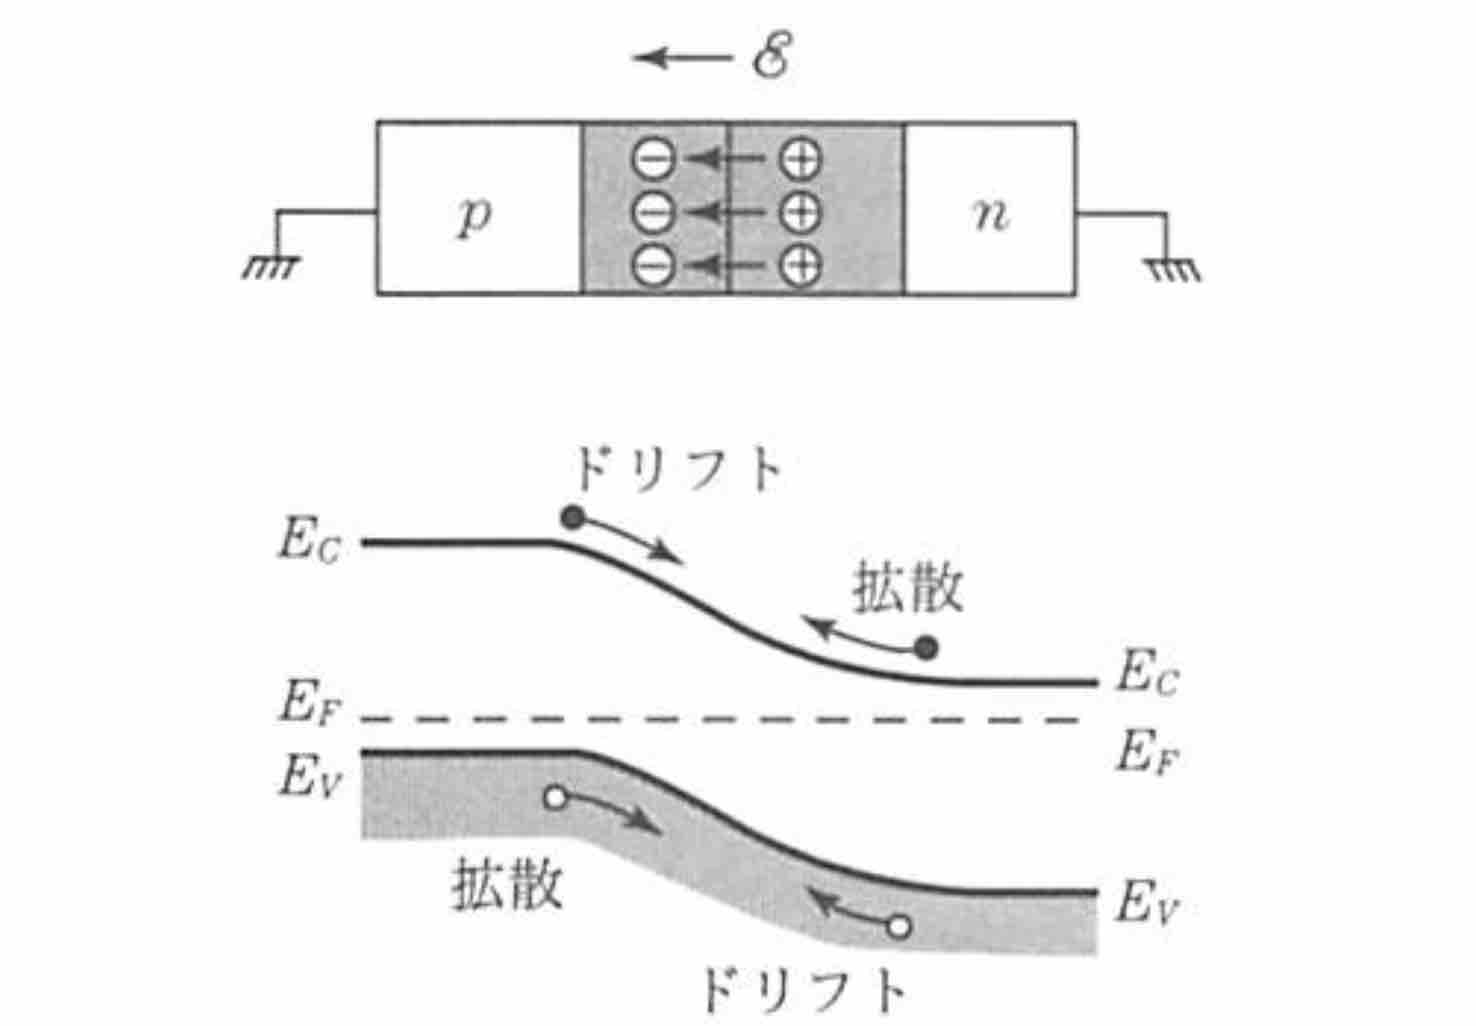
\includegraphics[width=6cm]{fig/ch2/pn.jpg}
    \caption[$pn$接合による電界形成の様子\cite{sze2012semiconductor}]{$pn$接合による電界形成の様子\cite{sze2012semiconductor}\\$n$型半導体の電子と$p$型半導体の正孔が拡散し、$n$側から$p$側へ電界が生じる。}
    \label{fg:pn}
\end{figure}

図\ref{fg:pn_bias} の(a)に$pn$接合の熱平衡状態の空乏層幅とエネルギーバンド図を示す。
空乏層幅が$W$で、$pn$接合のバンドギャップは電荷量を$q$、内蔵電位を$V_{\rm{bi}}$とすると$qV_{\rm{bi}}$と表せる。

\subsubsection{pn接合へ順バイアス電圧の印加}
$pn$接合の$p$側に順バイアス電圧を印加した時の空乏層の様子を 図\ref{fg:pn_bias} の(b)に示す。
$p$側へ$V_{\rm{F}}$の順バイアス電圧を印加すると、$pn$接合の電位は$V_{\rm{F}}$だけ下がるため、空乏層幅は 式\ref{eq:bulk} から減少することがわかる。
$pn$接合のバンドギャップも$q(V_{\rm{bi}}-V_{\rm{F}})$となり熱平衡状態のバンドギャップと比べて減少する。

\subsubsection{pn接合へ逆バイアス電圧の印加}
$pn$接合の$p$側に逆バイアス電圧を印加した時の空乏層の様子を 図\ref{fg:pn_bias} の(c)に示す。
$p$側へ$V_{\rm{R}}$の逆バイアス電圧を印加すると、pn接合の電位は$V_{\rm{R}}$だけ上昇するため、空乏層幅は 式\ref{eq:bulk} から増加することがわかる。
$pn$接合のバンドギャップも$q(V_{\rm{bi}}+V_{\rm{R}})$となり熱平衡状態のバンドギャップと比べて増加する。

\begin{figure}[h]
    \centering
    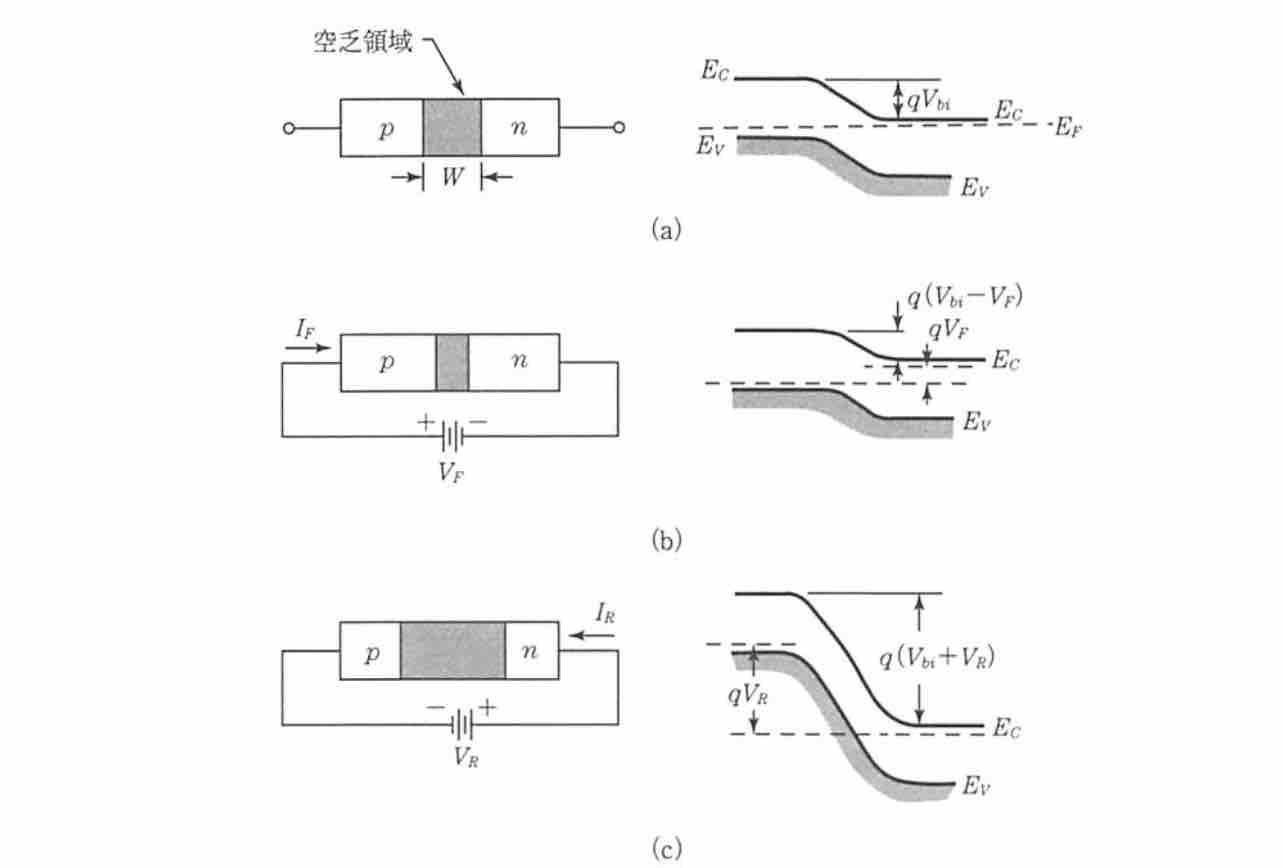
\includegraphics[width=12cm]{fig/ch2/pn_bias.jpg}
    \caption[熱平衡状態、順バイアス電圧、逆バイアス電圧におけるバルクの空乏層幅とエネルギーバンド図\cite{sze2012semiconductor}]{熱平衡状態、順バイアス電圧、逆バイアス電圧におけるバルクの空乏層幅とエネルギーバンド図\cite{sze2012semiconductor}\\(a)が熱平衡状態、(b)が順バイアス電圧、(c)が逆バイアス電圧の様子。}
    \label{fg:pn_bias}
\end{figure}

\subsection{電流電圧特性}
$pn$接合は特定の方向にだけ電流が流れやすい性質を持つ。
図\ref{fg:IV} に$pn$接合の電流電圧特性を示す。
$pn$接合に順バイアス電圧をかけると、$pn$接合のバンドギャップが減少し、キャリアがバンドギャップを越えることが容易になるため、電圧の増加とともに電流が急速に増加する。
逆バイアス電圧をかけると、$pn$接合のバンドギャップが増加するため、キャリアによる電流は流れない。
ある逆バイアスがある電圧に達すると大電流が流れる。
この電圧を降伏電圧と呼び、この電流は電子雪崩によって生じる電流である。

\begin{figure}[h]
    \centering
    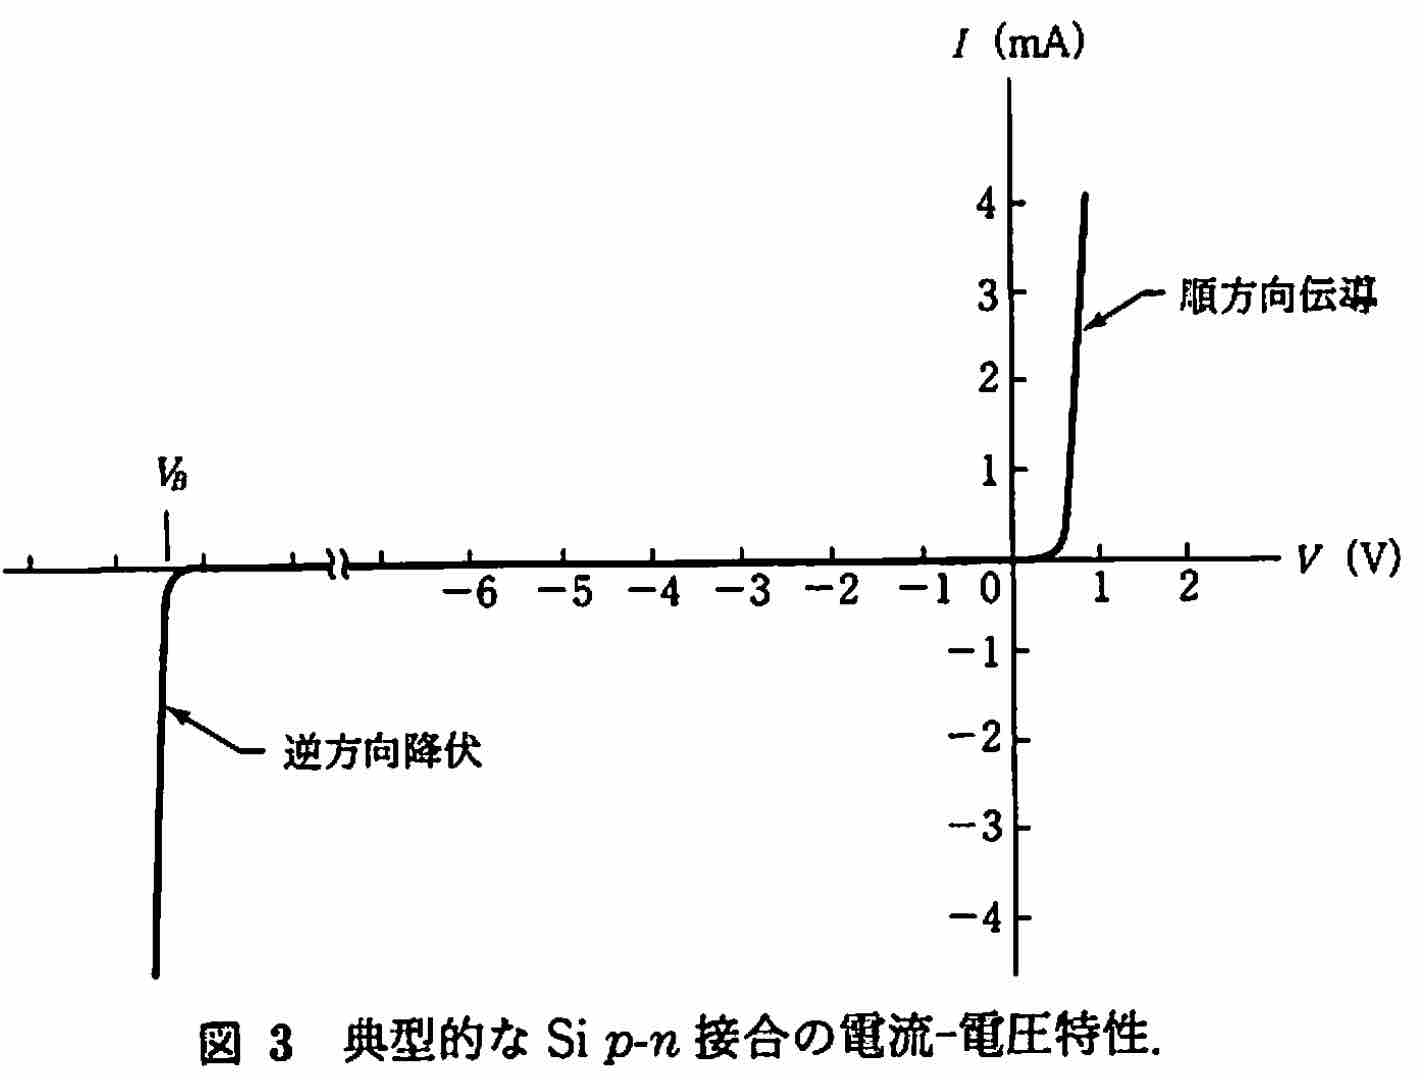
\includegraphics[width=8cm]{fig/ch2/IV.jpg}
    \caption[$pn$接合の電流電圧特性\cite{sze2012semiconductor}]{$pn$接合の電流電圧特性\cite{sze2012semiconductor}\\順バイアス電圧をかけると電圧上昇に伴い電流が上昇し、逆バイアス電圧をかけると降伏電圧で電流が上昇する。}
    \label{fg:IV}
\end{figure}



